\chapter{Riconoscitori LR}

\subsubsection{Parsing LR vs Parsing LL}
Costruendo l'albero top-down, la debolezza dell'analisi LL si traduce in:
\begin{itemize}
    \item deve poter identificare la produzione giusta usando soltanto i \textit{primi k simboli della parte destra}
    \item LL(1) è l'unico caso interessante
    \item LL(2) è utile in casi particolari
\end{itemize}

L'analisi LR invece, costruisce l'albero \textbf{bottom-up}:
\begin{itemize}
    \item parte dalle foglie, aspettando di avere abbastanza informazione per decidere come interpretarle
    \item meno naturale ma superiore dal punto di vista teorico
    \item ogni grammatica LL(k) è anche LR(k)
\end{itemize}

Tuttavia l'analisi LR è complessa da progettare e già il caso LR(1) spesso ingestibile per le grammatiche dei tipici linguaggi.

Sono state sviluppate \textit{tecniche semplificate}:
\begin{itemize}
    \item \textbf{SLR}: Simple LR
    \item \textbf{LALR}: Look-Ahead LR
\end{itemize}

Si utilizzano comunque sempre strumenti \textit{automatici}.

\begin{figure}[H]
    \caption{Gerarchia LR}
    \centering
    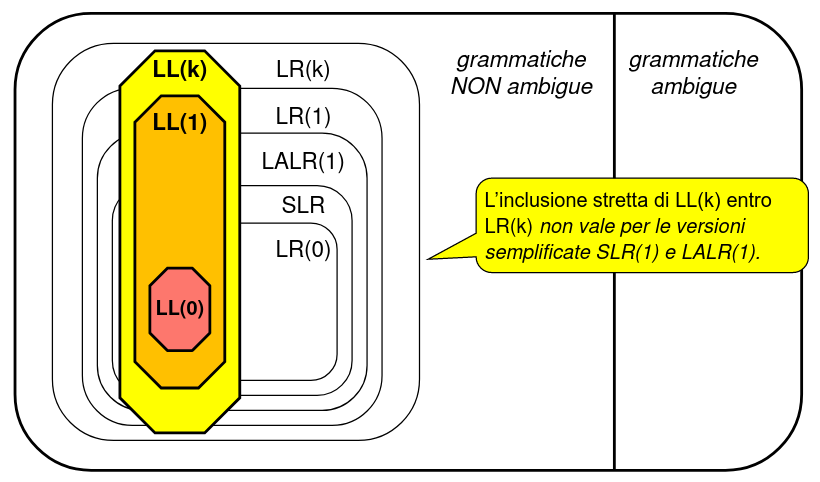
\includegraphics[width=0.7\textwidth]{/home/riccardoob/appunti/linguaggi/images/47.png}
\end{figure}

\subsubsection{Tecniche LR}
L'analisi LR procede BOTTOM UP, parte dalla frase e cerca di \textbf{riduarla} allo scopo S, ogni passo deve decidere se:
\begin{itemize}
    \item proseguire la lettura da input $\rightarrow$ \textbf{SHIFT}
    \item costruire un pezzo di albero $\rightarrow$ \textbf{REDUCE}
\end{itemize}

L'ultima REDUCE conclude l'albero con successo, accetta la frase nella fase di \textbf{ACCEPT}.

Per questo ha sempre bisogno di \textit{informazioni di contesto}.

\section{Architettura}
Il parser LR richiede un componenente, detto \textbf{ORACOLO}, che in base al contesto corrente, comunich se effettuare SHIFT o REDUCE al parser.

Un parser LR è quindi composto da:
\begin{itemize}
    \item un \textbf{oracolo}, che comunica se fare SHIFT o REDUCE
    \item uno \textbf{stack}, in cui conservare lo stato corrente di input e albero
    \item un \textbf{controller} che governa i primi due
\end{itemize}

\subsubsection{Informazione di contesto}
L'oracolo sfrutta opportune \textit{informazioni di contesto} per decidere se effettuare la lettura di un nuovo input o un passo di riduzione.

Questo componenente è un \textit{riconoscitore di contesti}, e solo se riconosce un appropriato \textit{contesto di riduzione}, ordina l'azione REDUCE appropriata per costruire senza ambiguità un certo pezzo di albero.

\section{Caso LR(0)}

Nell'analisi LR conviene studiare per prima LR(0), un sottoinsieme di LR nel quale è possibile scegliere la mossa da fare \textit{senza dover guardare il prossimo simbolo di input}.

In LR questo non significa non avere informazioni in assoluto, si precludono quelle future ma si ritengono informazioni sul contesto passato.

\subsection{Analisi LR(0)}
Passi:
\begin{itemize}
    \item calcolare il \textit{contesto} LR(0) di ciascuna produzione
    \item identificare \textbf{collisioni} in contesti di produzioni diverse
    \begin{itemize}
        \item \textbf{collisione}: stringa appartenente a un contesto è un \textbf{prefisso proprio} di una stringa in un altro contesto
        \item \textbf{prefisso proprio}: una stringa è prefisso di un'altra se ciò che segue è un terminale (non metasimbolo)
    \end{itemize}
    \item se non ci sono collisioni, si possono usare i contesti LR(0) per guidare l'analisi
\end{itemize}

Se sono presenti collisioni, i contesti LR(0) non sono sufficienti, è necessario testare con LR(1).
\subsubsection{Esempio 1}
Grammatica LR(0):
\setlist{nosep}
\begin{multicols}{2}
    \begin{itemize}
        \item \texttt{S} $\rightarrow$ \texttt{a A b}
        \item \texttt{S} $\rightarrow$ \texttt{a a B b a}
        \item \texttt{A} $\rightarrow$ \texttt{A a}
        \item \texttt{A} $\rightarrow$ \texttt{b}
        \item \texttt{B} $\rightarrow$ $\varepsilon$
    \end{itemize}
    \columnbreak
    \begin{itemize}
        \item[] contesto LR(0): \texttt{\{aAb\}}
        \item[] contesto LR(0): \texttt{\{aaBba\}}
        \item[] contesto LR(0): \texttt{\{aAa\}}
        \item[] contesto LR(0): \texttt{\{ab\}}
        \item[] contesto LR(0): \texttt{\{aa\}}
    \end{itemize}
\end{multicols}
\setlist{}

Da notare che non esiste collisione tra i contesti \texttt{aaBba} e \texttt{aa}, perché la stringa \texttt{aa}, pur essendo un prefisso di \texttt{aaBba} non è \textit{prefisso proprio} di quest'ultima (\texttt{B} è un non terminale).

La frase \texttt{abab} è analizzata come segue:

\begin{figure}[H]
    \centering
    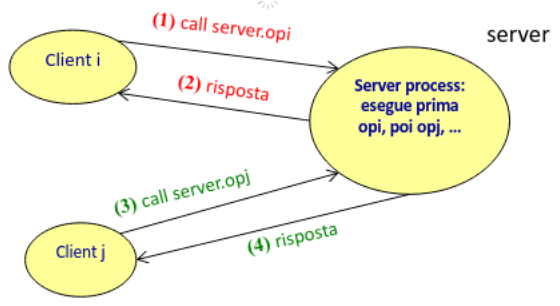
\includegraphics[width=\textwidth]{/home/riccardoob/appunti/linguaggi/images/48.png}
\end{figure}

Per ovviare a un possibile caso critico, conviene assumere che esista una produzione di \textbf{top-level} \texttt{Z} $\rightarrow$ \texttt{S}, dove \texttt{Z} è il nuovo scopo.

\subsubsection{Esempio 2}

\setlist{nosep}
\begin{multicols}{2}
    \begin{itemize}
        \item \texttt{S} $\rightarrow$ \texttt{a A b}
        \item \texttt{S} $\rightarrow$ \texttt{a a B b a}
        \item \texttt{A} $\rightarrow$ \texttt{A a}
        \item \texttt{A} $\rightarrow$ \texttt{b}
        \item \texttt{B} $\rightarrow$ $\varepsilon$
    \end{itemize}
    \columnbreak
    \begin{itemize}
        \item[] contesto LR(0): \texttt{\{aAb\}}
        \item[] contesto LR(0): \texttt{\{aaBba\}}
        \item[] contesto LR(0): \texttt{\{aAa\}}
        \item[] contesto LR(0): \texttt{\{ab\}}
        \item[] contesto LR(0): \texttt{\{aa\}}
    \end{itemize}
\end{multicols}
\setlist{}

La frase aaba è analizzata come segue:
\begin{figure}[H]
    \centering
    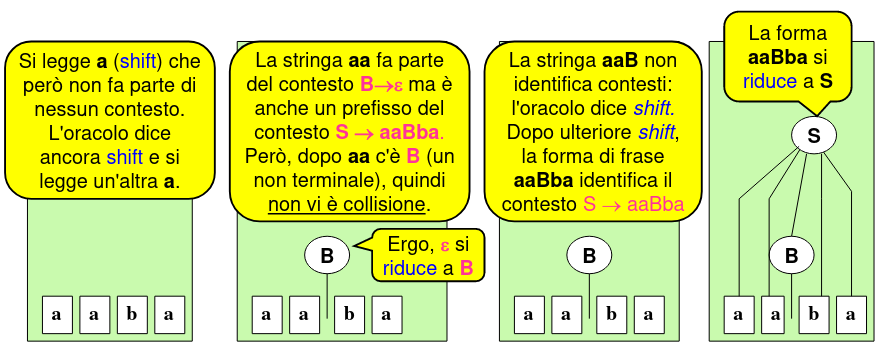
\includegraphics[width=\textwidth]{/home/riccardoob/appunti/linguaggi/images/49.png}
\end{figure}

L'emulatore richiede che la grammatica sia estesa con la regola top-level \texttt{Z} $\rightarrow$ \texttt{S}.

\subsubsection{Caso critico}
Perché il calcolo dei contesti può dare una informazione fuorviante se lo scopo è riuscato nella parte destra di qualche produzione?

Si consideri l'esempio:

\setlist{nosep}
\begin{multicols}{2}
    \begin{itemize}
        \item \texttt{S} $\rightarrow$ \texttt{S a}
        \item \texttt{S} $\rightarrow$ \texttt{a}
    \end{itemize}
    \columnbreak
    \begin{itemize}
        \item[] contesto LR(0): \texttt{\{Sa\}}
        \item[] contesto LR(0): \texttt{\{a\}}
    \end{itemize}
\end{multicols}
\setlist{}

Apparentemente i contesti sono diversi, tuttavia, dato che \texttt{S} può comparire in forme di frase intermedie, la "riduzione a \texttt{S}" non sempre denota il termine di una frase.

Aggiungere la regola top-level \texttt{Z} $\rightarrow$ \texttt{S} risolve l'ambiguità.

Supponendo di dover riconoscere la frase \texttt{aaa}:
\begin{itemize}
    \item senza la top-level, nella prima mossa si riduce \texttt{a} in \texttt{S}, ma poi non è chiaro se terminare o meno:
    \begin{itemize}
        \item se non ci sono altre \texttt{a}, si è già ridotto a \texttt{S}
        \item se la stringa continua con altre \texttt{a}, si applicano altre riduzione da S\texttt{Sa} ad \texttt{S}
        \item occorre tuttavia guardare avanti di un simbolo $\rightarrow$ no LR(0)
    \end{itemize}
    \item riformulando con lo scopo \texttt{Z}
    \setlist{nosep}
    \begin{multicols}{2}
        \begin{itemize}
            \item \texttt{Z} $\rightarrow$ \texttt{S}
            \item \texttt{S} $\rightarrow$ \texttt{S a}
            \item \texttt{S} $\rightarrow$ \texttt{a}
        \end{itemize}
        \columnbreak
        \begin{itemize}
            \item[] contesto LR(0): \texttt{\{S\}}
            \item[] contesto LR(0): \texttt{\{Sa\}}
            \item[] contesto LR(0): \texttt{\{a\}}
        \end{itemize}
    \end{multicols}
    \setlist{}
    \begin{itemize}
        \item si nota che i primi due contesti collidono
    \end{itemize}
\end{itemize}

\subsection{Contesti LR(0)}
Il calcolo dei contesti LR(0) si basa sul fatto che essi sono definiti da una \textit{opportuna grammatica}.
\begin{mdframed}[topline=false,bottomline=false,rightline=false]
La grammatica che definisce i contesti LR(0) è sempre \textbf{regolare} (a sinistra).
\end{mdframed}

Ciò denota che il \textit{riconoscimento del contesto corrente}, svolto dall'oracolo, si può ottenere con un \textit{automa a stati finiti}. 

\subsubsection{Definizione}
\begin{mdframed}[topline=false,bottomline=false,rightline=false]
Il contesto LR(0) di una produzione \texttt{A} $\rightarrow$ $\alpha$\\
$\text{LR(0) ctx(\text{A}} \rightarrow \alpha) = \{\gamma | \gamma = \beta\alpha, \text{Z}\Rightarrow \beta\text{Aw} \Rightarrow \beta \alpha \text{w}, \text{w} \in \text{VT*}\}$
\end{mdframed}

Tradotto:
\begin{mdframed}[topline=false,bottomline=false,rightline=false]
Il contesto LR(0) della produzione \texttt{A} $\rightarrow$ $\alpha$ è l'insieme di tutti i \textbf{prefissi} ($\beta\alpha$) di una forma di frase che usi la produzione \texttt{A} $\rightarrow$ $\alpha$ all'ultimo passo ($\beta\alpha\text{w} \Rightarrow \beta\alpha\text{w}$) di una derivazione canonica destra.
\end{mdframed}
Conseguenza:
\begin{mdframed}[topline=false,bottomline=false,rightline=false]
Tutte le stringhe del contesto LR(0) della produzione \texttt{A} $\rightarrow$ $\alpha$ hanno la forma $\alpha\beta$ e \textit{differiscono solo per il prefisso} $\beta$.
\end{mdframed}

\subsubsection{Calcolo}
Dato che le stringhe del contesto LR(0) differiscono solo per il prefisso $\beta$, che dipende da \texttt{A}, si può esprimere il contesto come concatenazione tra insieme dei $\beta$ e il suffisso $\alpha$.

L'insieme dei $\beta$ si chiama \textbf{contesto sinistro} di \texttt{A}.

Formalmente:
\begin{mdframed}[topline=false,bottomline=false,rightline=false]
Il contesto sinistro di un non terminale \texttt{A}:
\begin{equation*}
    \text{leftctx(A)} = \{\beta | \text{Z} \Rightarrow \beta\text{Aw}, \text{w} \in \text{VT*}\}
\end{equation*}
da cui il contesto LR(0) della produzione \texttt{A} $\rightarrow$ $\alpha$
\begin{equation*}
    \text{LR(0) ctx(A}\rightarrow\alpha) = \text{leftctx(A)} \cdot \{\alpha\}
\end{equation*}
\end{mdframed}

\subsubsection{Calcolo dei contesti sinistri}
Determinare leftctx(\texttt{A}), comporta trovare tutti i modi in cui può apparire il metasimbolo \texttt{A} in una forma di frase.

Poiché lo scopo \texttt{Z} per definizione non compare mai nella parte destra di alcuna produzione, leftxctx(\texttt{Z}) = $\{ \varepsilon \}$.

Data una produzione \texttt{B} $\rightarrow$ $\gamma \texttt{A} \delta$, i prefissi che possono esserci davanti ad \texttt{A} sono quelli che potevano esserci davanti a \texttt{B} seguiti dalla stringa $\gamma$.

Un primo contributo a leftctx(\texttt{A}) è
\begin{equation*}
    \text{leftctx(\texttt{A})} \supseteq \text{leftctx(\texttt{B})} \cdot \{\gamma\}
\end{equation*}

Si analizzano poi tutte le altre produzioni nelle quali compare \texttt{A} nella parte destra.

\subsubsection{Esempio}

\setlist{nosep}
\begin{itemize}
    \item \texttt{Z} $\rightarrow$ \texttt{S}
    \item \texttt{S} $\rightarrow$ \texttt{a S A B | B A}
    \item \texttt{A} $\rightarrow$ \texttt{a A | B}
    \item \texttt{B} $\rightarrow$ \texttt{b}
\end{itemize}
\setlist{}

Considerando i due postulati:
\begin{align*}
    &\text{leftctx(\texttt{Z})} = \{ \varepsilon \}\\
    &\texttt{B} \rightarrow \gamma \texttt{A} \delta \Rightarrow \text{leftctx(\texttt{A})} \supseteq \text{leftctx(\texttt{B})} \cdot \{\gamma\}
\end{align*}

Postulato 1 e 2 per produzione \texttt{Z} $\rightarrow$ \texttt{S}
\setlist{nosep}
\begin{itemize}
    \item leftctx(\texttt{Z}) = \{$\varepsilon$\}
    \item leftctx(\texttt{S}) $\supseteq$ leftctx(\texttt{Z}) $\cdot \{\varepsilon\}$ = leftctx(\texttt{Z})
\end{itemize}
\setlist{}

Postulato 2 per la produzione \texttt{S} $\rightarrow$ \texttt{a S A B | B A}
\setlist{nosep}
\begin{multicols}{2} 
    \begin{itemize}
        \item leftctx(\texttt{S}) $\supseteq$ leftctx(\texttt{S}) $\cdot \{\texttt{a}\}$
        \item leftctx(\texttt{A}) $\supseteq$ leftctx(\texttt{S}) $\cdot \{\texttt{aS}\}$
        \item leftctx(\texttt{B}) $\supseteq$ leftctx(\texttt{S}) $\cdot \{\texttt{aSA}\}$
        \item leftctx(\texttt{B}) $\supseteq$ leftctx(\texttt{S}) $\cdot \{\varepsilon\}$
        \item leftctx(\texttt{A}) $\supseteq$ leftctx(\texttt{S}) $\cdot \{\texttt{B}\}$
    \end{itemize}
    \columnbreak
    \begin{itemize}
        \item[] (\texttt{S} $\rightarrow$ \texttt{a S} $\delta$)
        \item[] (\texttt{S} $\rightarrow$ \texttt{a S A} $\delta$)
        \item[] (\texttt{S} $\rightarrow$ \texttt{a S A B})
        \item[] (\texttt{S} $\rightarrow$ \texttt{B} $\delta$)
        \item[] (\texttt{S} $\rightarrow$ \texttt{B A})
    \end{itemize}
\end{multicols}
\setlist{}

Postulato 2 per la produzione \texttt{A} $\rightarrow$ \texttt{a A | B}
\setlist{nosep}
\begin{multicols}{2} 
    \begin{itemize}
        \item leftctx(\texttt{A}) $\supseteq$ leftctx(\texttt{A}) $\cdot \{\texttt{a}\}$
        \item leftctx(\texttt{B}) $\supseteq$ leftctx(\texttt{A}) $\cdot \{\varepsilon\}$
    \end{itemize}
    \columnbreak
    \begin{itemize}
        \item[] (\texttt{A} $\rightarrow$ \texttt{a A})
        \item[] (\texttt{A} $\rightarrow$ \texttt{B})
    \end{itemize}
\end{multicols}
\setlist{}

Componendo i pezzi
\setlist{nosep}
\begin{multicols}{2}
    \begin{itemize}
        \item leftctx(\texttt{Z}) = \{$\varepsilon$\}
        \item[]
        \item leftctx(\texttt{S}) $\supseteq$ leftctx(\texttt{Z})
        \item leftctx(\texttt{S}) $\supseteq$ leftctx(\texttt{S}) $\cdot$ \{\texttt{a}\}
        \item[]
        \item leftctx(\texttt{A}) $\supseteq$ leftctx(\texttt{S}) $\cdot$ \{\texttt{aS}\}
        \item leftctx(\texttt{A}) $\supseteq$ leftctx(\texttt{S}) $\cdot$ \{\texttt{B}\}
        \item leftctx(\texttt{A}) $\supseteq$ leftctx(\texttt{A}) $\cdot$ \{\texttt{a}\}
        \item[]
        \item leftctx(\texttt{B}) $\supseteq$ leftctx(\texttt{S}) $\cdot$ \{\texttt{aSA}\}
        \item leftctx(\texttt{B}) $\supseteq$ leftctx(\texttt{S})
        \item leftctx(\texttt{B}) $\supseteq$ leftctx(\texttt{A})
    \end{itemize}
    \columnbreak
    \begin{itemize}
        \item[] leftctx(\texttt{Z}) = \{$\varepsilon$\}
        \item[]
        \item[] leftctx(\texttt{S}) = leftctx(\texttt{Z}) $\cup$
        \item[] \makebox[2.16cm]{}    leftctx(\texttt{S}) $\cdot$ \{\texttt{a}\}
        \item[]
        \item[] leftctx(\texttt{A}) = leftctx(\texttt{S}) $\cdot$ \{\texttt{aS}\} $\cup$
        \item[] \makebox[2.16cm]{}    leftctx(\texttt{S}) $\cdot$ \{\texttt{B}\} $\cup$
        \item[] \makebox[2.16cm]{}    leftctx(\texttt{A}) $\cdot$ \{\texttt{a}\}
        \item[]
        \item[] leftctx(\texttt{B}) = leftctx(\texttt{S}) $\cdot$ \{\texttt{aSA}\} $\cup$
        \item[] \makebox[2.16cm]{}    leftctx(\texttt{S}) $\cup$
        \item[] \makebox[2.16cm]{}    leftctx(\texttt{A})
    \end{itemize}
\end{multicols}
\setlist{}
\newpage
\setlist{nosep}
\begin{multicols}{2}
    \begin{itemize}
        \item leftctx(\texttt{Z}) = \{$\varepsilon$\}
        \item[]
        \item leftctx(\texttt{S}) = leftctx(\texttt{Z}) $\cup$
        \item \makebox[2.16cm]{}    leftctx(\texttt{S}) $\cdot$ \{\texttt{a}\}
        \item[]
        \item leftctx(\texttt{A}) = leftctx(\texttt{S}) $\cdot$ \{\texttt{aS}\} $\cup$
        \item \makebox[2.16cm]{}    leftctx(\texttt{S}) $\cdot$ \{\texttt{B}\} $\cup$
        \item \makebox[2.16cm]{}    leftctx(\texttt{A}) $\cdot$ \{\texttt{a}\}
        \item[]
        \item leftctx(\texttt{B}) = leftctx(\texttt{S}) $\cdot$ \{\texttt{aSA}\} $\cup$
        \item \makebox[2.16cm]{}    leftctx(\texttt{S}) $\cup$
        \item \makebox[2.16cm]{}    leftctx(\texttt{A})
    \end{itemize}
    \columnbreak
    \begin{itemize}
        \item[] $\langle$\texttt{LctxZ}$\rangle \rightarrow \{\varepsilon\}$
        \item[]
        \item[] $\langle$\texttt{LctxZ}$\rangle \rightarrow \langle$LctxZ$\rangle$ $|$
        \item[] \makebox[1.97cm]{}    $\langle$\texttt{LctxS}$\rangle$ \texttt{a}
        \item[]
        \item[] $\langle$\texttt{LctxS}$\rangle \rightarrow \langle$LctxS$\rangle$ \texttt{aS} $|$
        \item[] \makebox[1.97cm]{}    $\langle$\texttt{LctxS}$\rangle$ \texttt{B} $|$
        \item[] \makebox[1.97cm]{}    $\langle$\texttt{LctxA}$\rangle$ \texttt{a}
        \item[]
        \item[] $\langle$\texttt{LctxB}$\rangle \rightarrow \langle$LctxS$\rangle$ \texttt{aSA} $|$
        \item[] \makebox[1.97cm]{}    $\langle$\texttt{LctxS}$\rangle$ $|$
        \item[] \makebox[1.97cm]{}    $\langle$\texttt{LctxA}$\rangle$
    \end{itemize}
\end{multicols}
\setlist{}

Risolvendo le equazioni si possono trovare le espressioni regolari dei vari contesti:
\setlist{nosep}
\begin{itemize}
    \item leftctx(\texttt{Z}) = \{$\varepsilon$\}
    \item leftctx(\texttt{S}) = \{\texttt{a*}\}
    \item leftctx(\texttt{A}) = \{\texttt{(a* a S + a* B) a*}\}
    \item leftctx(\texttt{B}) = \{\texttt{a* a S A + a* + (a* a S + a* B) a*}\}
\end{itemize}
\setlist{}

Semplificando le espressioni regolari
\setlist{nosep}
\begin{itemize}
    \item leftctx(\texttt{Z}) = \{$\varepsilon$\}
    \item leftctx(\texttt{S}) = \{\texttt{a*}\}
    \item leftctx(\texttt{A}) = \{\texttt{a*(a S + B) a*}\}
    \item leftctx(\texttt{B}) = \{\texttt{a* (a S A + $\varepsilon$) + a* (a S + B) a*}\}
\end{itemize}
\setlist{}
e concatenando i contesti sinistri con i rispettivi suffissi
\setlist{nosep}
\begin{itemize}
    \item LR(0)ctx(\texttt{Z} $\rightarrow$ \texttt{S}) = \{$\varepsilon$\} \texttt{S} = \{\texttt{S}\}
    \item LR(0)ctx(\texttt{S} $\rightarrow$ \texttt{aSAB}) = \{\texttt{a*aSAB}\}
    \item LR(0)ctx(\texttt{S} $\rightarrow$ \texttt{BA}) = \{\texttt{a*BA}\}
    \item LR(0)ctx(\texttt{A} $\rightarrow$ \texttt{aA}) = \{\texttt{a*(aS+B)a*aA}\}
    \item LR(0)ctx(\texttt{A} $\rightarrow$ \texttt{B}) = \{\texttt{a*(aS+B)a*B}\}
    \item LR(0)ctx(\texttt{B} $\rightarrow$ \texttt{b}) = \{\texttt{a*(aSA+$\varepsilon$)b+a*(aS+B)a*b}\}
\end{itemize}
\setlist{}
si ottengono diversi linguaggi, è necessario costruire un RSF che riconosca l'unione di questi linguaggi: è necessario che risulti \textbf{deterministico}.

\subsection{L'automa a stati ausiliario}
Questo RSF è la \textbf{macchina caratteristica} della grammatica iniziale: ogni stato finale è etichettato con una produzione, usata dal parser per effettuare una REDUCE nel contesto.

Si parte ogni volta dallo stato iniziale e si percorre l'ASF per deciedere la mossa.

\begin{figure}[H]
    \centering
    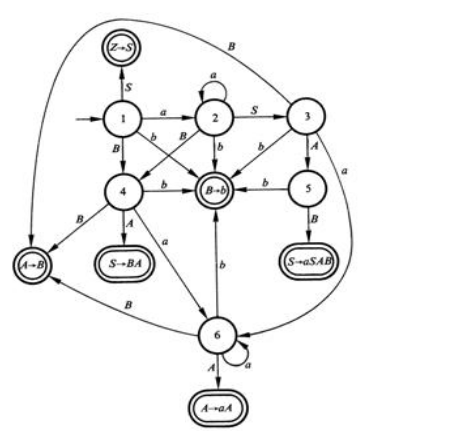
\includegraphics[width=0.6\textwidth]{/home/riccardoob/appunti/linguaggi/images/50.png}
\end{figure}

\subsubsection{Algoritmo parsing LR(0)}
L'analisi LR(0) di una frase si svolge sottoponendo all'automa carrateristico la forma di frase corrente.

\begin{itemize}
    \item \textbf{SHIFT}: quando l'automa caratteristico raggiunge uno stato \textit{non finale}, indica che le informazioni disponibili non sono sufficienti
    \item \textbf{REDUCE}: quando l'automa caratteristico raggiunge uno stato \textit{finale}, si applica quindi la produzione raggiunta
\end{itemize}

La forma di frase corrente è mantenuta su uno stack:
\begin{itemize}
    \item \textbf{SHIFT} pone in \textit{cima} allo stack il nuovo simbolo terminale letto
    \item \textbf{REDUCE} \textit{toglie} dallo stack tanti elementi quanti sono quelli nella \textit{parte destra} della produzione da applicare e si pone in \textit{cima} allo stack il simbolo non terminale corrispondente alla \textit{parte sinistra} di tale riduzione.
\end{itemize}

ESEMPIO A SLIDE 40-43

\subsubsection{Miglioramenti}
Ogni volta che si effettua una REDUCE si riparte dallo stato iniziale, ma dato che la forma di frase cambia solo in fondo anche la prima parte del percorso non cambia.

Si può quindi ottimizzare il processo memorizzando il percorso fatto, ripartendo dall'ultimo stato utile; a questo scopo si utilizza uno \textit{stack ausiliario degli stati}, dove si impilano gli stati attraversati e se ne rimuovono tanti quanti i simboli coinvolti in un passo di riduzione.

ESEMPIO SLIDE 45-51

\subsection{Condizione LR(0)}
\begin{mdframed}[topline=false,bottomline=false,rightline=false]
Condizione sufficiente perché una grammatica sia LR(0) è che, date due produzioni \texttt{A} $\rightarrow \alpha$ e \texttt{B} $\rightarrow \omega$
\begin{itemize}
    \item se $\theta \in$ LR(0)(ctx\texttt{A}$ \rightarrow \alpha$) dove $\theta \in (\texttt{VT} \cup \texttt{VN})*$
    \item e $\theta $w$ \in$ LR(0)ctx(\texttt{B}$ \rightarrow \omega$) dove w $\in$ \texttt{VT}*
\end{itemize}
risulti
\begin{equation*}
    \text{w} = \varepsilon, \text{A} = \text{B}, \alpha = \omega
\end{equation*}

Ogni stato di riduzione dell'automa ausiliario sia etichettato da una \textit{produzione unica} e \textit{non abbia archi di uscita} etichettati da terminali.
\end{mdframed}

\subsection{Automa caratteristico - approccio alternativo}
Il metodo descritto è difficile da automatizzare e complesso, esiste tuttavia un metodo operativo facilmente meccanizzabile.

\subsubsection{Procedimento operativo}
Si parte dalla regola top-level \texttt{Z} $\rightarrow$ \texttt{S\$} e si analizzano le situazioni che si presentano:
\begin{itemize}
    \item creare un rettangolo \textbf{LR item} per ogni "situazione"
    \item quando una regola ne usa un'altra, la includiamo nel corrispondente LR item
    \item si introduce l'astrazione di \textbf{cursore "."} che indica la posizione all'interno della regola dell'analisi
\end{itemize}

Si studiano le evoluzioni possibili di ogni LR item, costruendo l'automa dal basso, caso per caso.

\paragraph{Convenzioni}
\begin{itemize}
    \item ogni frase lecita è terminata da \texttt{\$}
    \item il \textit{cursore} \texttt{.} denota il \textit{confine} tra la parte già analizzata e quella ancora da analizzare: \texttt{A} $\rightarrow$ \texttt{a.B}, il prossimo input è \texttt{B}, dove
    \begin{itemize}
        \item \textit{input} è la forma di frase eventualmente già sottoposta a passi di riduzione (simboli terminali e non terminale della grammatica di partenza)
        \item l'automa si appoggia allo stack di input: i simboli a sinistra del cursore sono già stati estratti, l'\textit{input è il simbolo al top dello stack}
    \end{itemize}
\end{itemize}
Facendo riferimento alla grammatica
\setlist{nosep}
\begin{itemize}
    \item \texttt{Z} $\rightarrow$ \texttt{S}
    \item \texttt{S} $\rightarrow$ \texttt{a S A B | B A}
    \item \texttt{A} $\rightarrow$ \texttt{a A | B}
    \item \texttt{B} $\rightarrow$ \texttt{b}
\end{itemize}
\setlist{}
Tutti gli input sono ancora da leggere e ogni frase lecita deriva dallo scopo Z:
\setlist{nosep}
\begin{itemize}
    \item \texttt{Z} $\rightarrow$ \texttt{.S\$}
\end{itemize}
\setlist{}

Per descrivere appieno questo stato, occorre specificare anche tutte le produzioni di \texttt{S}

\setlist{nosep}
\begin{itemize}
    \item \texttt{Z} $\rightarrow$ \texttt{.S\$}
    \item \texttt{S} $\rightarrow$ \texttt{.aSAB | .BA}
    \item \texttt{B} $\rightarrow$ \texttt{.b}
\end{itemize}
\setlist{}

Si include anche \texttt{B} poiché una delle produzioni di \texttt{S} può iniziare \texttt{B}.

Una volta individuato un stato, in questo caso stato \texttt{\underline{1}}, si procede a analizzare tutte le possibili evoluzioni spostando il cursore a \textit{destra in tutti i modi possibili}:

\begin{itemize}
    \item con input \texttt{S}, situazione \texttt{Z} $\rightarrow$ \texttt{S.\$}
    \item con input \texttt{a}, situazione \texttt{S} $\rightarrow$ \texttt{a.SAB}
    \item con input \texttt{B}, situazione \texttt{S} $\rightarrow$ \texttt{B.A}
    \item con input \texttt{b}, situazione \texttt{B} $\rightarrow$ \texttt{b.}
\end{itemize}
Si denotano due stati finali
\begin{itemize}
    \item situazione \texttt{Z} $\rightarrow$ \texttt{S.\$}, stato finale di accettazione \texttt{\underline{F}}
    \item situazione \texttt{B} $\rightarrow$ \texttt{b.}, stato finale di riduzione \texttt{\underline{R1}}
\end{itemize}

Nella situazione \texttt{S} $\rightarrow$ \texttt{a.SAB} (stato \texttt{\underline{2}}), l'input può iniziare per \texttt{S}, quindi vanno considerate tutte le produzioni relative a \texttt{S}, tra queste una può iniziare per \texttt{B} quindi si aggiunge anche \texttt{B} $\rightarrow$ \texttt{b}, si ottiene lo stato \texttt{\underline{2}}
\setlist{nosep}
\begin{itemize}
    \item \texttt{S} $\rightarrow$ \texttt{a.SAB}
    \item \texttt{S} $\rightarrow$ \texttt{.aSAB | .BA}
    \item \texttt{B} $\rightarrow$ \texttt{.b}
\end{itemize}
\setlist{}




























































